\documentclass[12pt, a4paper]{article}
\usepackage[UTF8]{ctex}
\usepackage{amsmath}
\usepackage{amssymb}
\usepackage{amsthm}
\usepackage{geometry}
\usepackage{enumitem}
\usepackage{indentfirst}
\usepackage{caption}
\usepackage{fancyhdr}
\usepackage{booktabs}
\usepackage{titlesec}
\usepackage{draftwatermark}%水印
\usepackage{graphicx} % 导入图像的宏包、单图
% 页面布局设置
\geometry{top=2.54cm, bottom=2.54cm, left=3.18cm, right=3.18cm}

\SetWatermarkText{B站：布加拉提}
\SetWatermarkScale{0.4}

% 行距设置
\linespread{1.5}

% 段落设置
\setlength{\parindent}{2em}
\setlength{\parskip}{0.5em}

% 节标题格式设置
\titleformat{\section}{\normalfont\Large\bfseries}{第\chinese{section}章、}{1em}{}
\titlespacing{\section}{0pt}{2.5ex plus 1ex minus .2ex}{1.3ex plus .2ex}

% 定理环境设置
\newtheoremstyle{solution}
{}
{}
{}
{}
{\bfseries}
{、}
{1em}
{}
\theoremstyle{solution}
\newtheorem{sol}{解}

% 页眉页脚设置
\pagestyle{fancy}
\fancyhf{}
\fancyhead[C]{b站布加拉提整理（回忆版）b站甘茶w独家讲解}
\fancyfoot[C]{\thepage}

\rfoot{整理人：八方\\资源提供：考研乔瑟夫}
\lhead{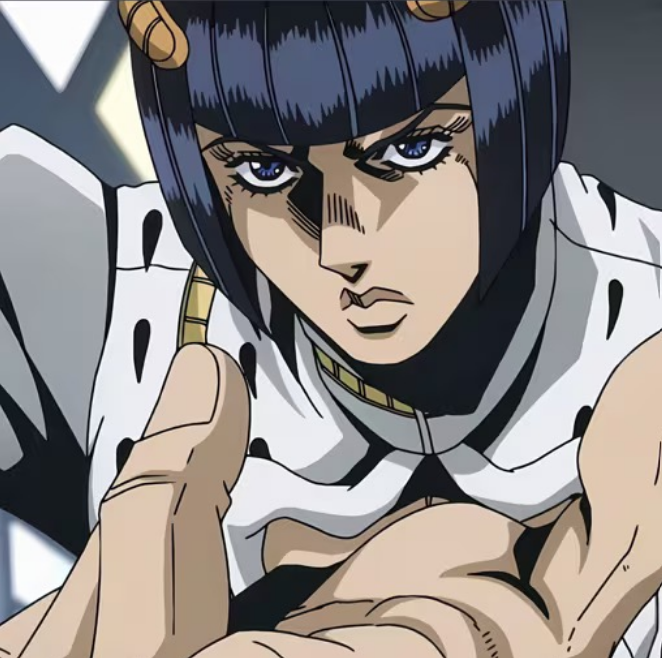
\includegraphics[width=0.06\linewidth]{p1.png}}
\rhead{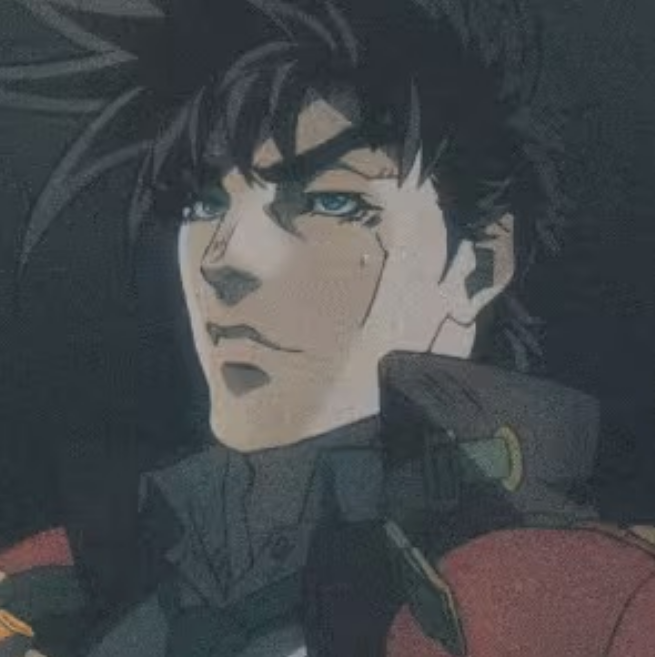
\includegraphics[width=0.06\linewidth]{p2.png}}
\renewcommand{\headrulewidth}{0.4pt}
\renewcommand{\footrulewidth}{0.4pt}

\begin{document}

\begin{center}
\Large\textbf{2024哈工大硕士考试试题：805物理光学}
\end{center}





\section*{一、填空题}
\begin{enumerate}
    \item 三个物质方程
    \item 以布儒斯特角入射，反射光的偏振状态
    \item 正常色散，反常色散对应吸收曲线的哪一部分
    \item 干涉的必要条件和补充条件
    \item 圆形相干面积公式
    \item 波带片有几个
    \item 负单轴晶体，比o光和e光速度，光轴在哪里
\end{enumerate}
\section*{二、选择题}
\begin{enumerate}
    \item 两个平行为I的光，最大光强是
    A.I\quad B.2I\quad C.3I\quad D.4I
    \item 光栅的分辨本领
    A.正比于光栅总刻线数\quad B.反比于光栅总刻度线\quad C.正比于光栅常数\quad D.反比于光栅常数
    \item 杨氏双缝，两小孔之间的距离超过了横向相干宽度
    A.0\quad D.一会大一会小，总体趋向稳定
    \item 两个结构相同的激光
    A.相干\quad B.不一定相干\quad C.不相干
    \item 电光效应的根本原因
    A.改变了光场的本质\quad B.改变了介质的性质
    \item 法布里-波罗标准具用来
    A.测量长度 \quad B.研究谱线
\end{enumerate}
\section*{三、名词解释}
\begin{enumerate}
    \item 倏逝波
    \item 惠更斯-菲涅尔原理
    \item 吸收定律
    \item 法拉第效应
    \item 光栅
    \item 菲涅尔波带片
    \item 偏振度
\end{enumerate}
\section*{四、简答题}
\begin{enumerate}
    \item 是什么光，是否单色光，各自的强度和合成强度分别为多少\\
    $E_x=Asin(wt-kz+\frac{\pi}{2}),E_y=Acos(wt-kz-\frac{\pi}{2})$\\
    $E_x=Acos(wt-kz+\varphi _x(t)),E_y=Acos(wt-kz+\varphi_y(t))$\\
    其中$\varphi _y(t)-\varphi _x(t)\neq 常数$
    \item 全反射的条件，入射角大于临界角时，反射光的偏振特性
    \item 比较圆形等倾条纹和牛顿环的异同，空气层改变时怎么变化
    \item 条纹对比度和哪些因素有关，简述空间相干性和时间相干性与个因素的关系
    \item 比较棱镜与光栅的色分辨本领的区别
    \item 瑞利散射的特点
\end{enumerate}
\section*{五、计算题}
\begin{enumerate}
    \item 用光程差$(n-1)d $大于等于波列长度，什么情况下相干
    \item 迈克尔逊干涉仪，中央是一个亮斑，可以看到20条亮条纹，移动距离，减少了20条，还可以看到10条
        \begin{enumerate}
            \item 移动前中央暗斑的级次
            \item 移动后第五个暗斑的角半径
        \end{enumerate}
    \item 自然光和圆偏振光，通过1/4波片和偏振片，最大光强是最小光强的七倍，问自然光占部分偏振光的百分之多少？
    \item 光栅$a=0.001mm$，每毫米有200缝，光栅昌都$5cm$
        \begin{enumerate}
            \item 能否区别$500nm$和$500.02nm$的两条光
            \item 哪几条缺级
        \end{enumerate}
    \item 牛顿环，波长为$\lambda_1$的第5条与某一波长的第七条重合，问波长
\end{enumerate}
\section*{六、论述题}
\begin{enumerate}
    \item 比较法布里-波罗干涉仪和光栅的各种性能指标
\end{enumerate}
\end{document}